\documentclass{TheMartianReport}
\usepackage[english]{babel}
\usepackage[utf8]{inputenc}
\usepackage[T1]{fontenc}

\usepackage[onehalfspacing]{setspace}
\usepackage{microtype}


\usepackage{amsmath,amssymb,amstext}
\usepackage{float}
%\usepackage{subfig}
\usepackage{subcaption}
\usepackage{graphicx}
\usepackage{picinpar}
\usepackage{wrapfig}
\usepackage{hyperref} % Für die Verwendung von URLs
\usepackage{gensymb}
%\usepackage[automark]{scrpage2}
%\usepackage[stable]{footmisc} % Für Fußnoten in Sections
\usepackage[normalem]{ulem}


\usepackage{multirow}
\usepackage{pdfpages}
\usepackage{lipsum}  
\usepackage[rightcaption]{sidecap}

\usepackage{framed}
\usepackage{calrsfs}
\DeclareMathAlphabet{\pazocal}{OMS}{zplm}{m}{n}

\usepackage[superscript,nomove]{cite}


%\bibliographystyle{ieeetr}

% Corrections and remarks
\usepackage{xcolor}
\usepackage[normalem]{ulem}

% For comparing corrections
%\newcommand{\red}[1]{{\color{red} #1}}          % add
%\newcommand{\blue}[1]{{\color{blue} \sout{#1}}} % remove
%\newcommand{\green}[1]{{\color{green} #1}}      % comment

% For final version after revision 1
\newcommand{\red}[1]{#1} % add
\newcommand{\blue}[1]{}  % remove
\newcommand{\green}[1]{} % comment

% Revision 2
%\newcommand{\redx}[1]{{\color{red} #1}}          % add
%\newcommand{\bluex}[1]{{\color{blue} \sout{#1}}} % remove
%\newcommand{\greenx}[1]{{\color{green} #1}}      % comment

% For final version after revision 2
\newcommand{\redx}[1]{#1} % add
\newcommand{\bluex}[1]{}  % remove
\newcommand{\greenx}[1]{} % comment

%%%%%%%%%%%%%%%%%%%%%% COVER PAGE VALUES %%%%%%%%%%%%%%%%%%%%%%
\title{GORILLA} % Change document title
\author{Michael Eder} % Change author name
\project{Guiding-center ORbit Integration with Local Linearization Approach} % Change (or omit) project name
%\date{} % Change displayed date value from default
\imagefolder{./figures} % Change folder to look for images in
\logo{title_image.eps} % Add logo image to cover page
\revision{Revision 1.0} % Change revision number

%%%%%%%%%%%%%%%%%%%%%%% GENERAL SETTINGS %%%%%%%%%%%%%%%%%%%%%%%
%\bibliographystyle{abbrvnat} % Change bibliography style
%\footertext{}{} % Change values in footer text
%\nofootertext % Hide footer text
\drafting % Comment out to hide \temp and \crit sections
\sectionnumbers% Sections are major numbers, subsections minor, etc.
%\subsectionnumbers % Sections not numbered, only begin at subsections and below

%%%%%%%%%%%%%%%%%%%%%%%%%%%%%%%%%%%%%%%%%%%%%%%%%%%%%%%%%%%%%%%%%%%%%%%%%%
\begin{document}

%\printhelp % Use this to see/print help pages

\newcommand{\be}[1]{\begin{equation} \label{#1}}
\newcommand{\ee}{\end{equation}}
\newcommand{\bea}[1]{\begin{eqnarray} \label{#1}}
\newcommand{\eea}{\end{eqnarray}}
\newcommand{\bean}{\begin{eqnarray*}}
\newcommand{\eean}{\end{eqnarray*}}
\newcommand{\non}{\nonumber\\}
\newcommand{\eq}[1]{(\ref{#1})}
\newcommand{\difp}[2]{\frac{\partial #1}{\partial #2}}
\newcommand{\bA}{{\textbf{A}}}
\newcommand{\ba}{{\bf a}}
\newcommand{\bB}{{\textbf{B}}}
\newcommand{\bb}{{\bf b}}
\newcommand{\bE}{{\textbf{E}}}
\newcommand{\bG}{{\textbf{G}}}
\newcommand{\bn}{{\textbf{n}}}
\newcommand{\bN}{{\textbf{N}}}
\newcommand{\bp}{{\textbf{p}}}
\newcommand{\bP}{{\textbf{P}}}
\newcommand{\bR}{{\bf R}}
\newcommand{\bV}{{\textbf{V}}}
\newcommand{\bX}{{\textbf{X}}}
\newcommand{\bY}{{\textbf{Y}}}
\newcommand{\bZ}{{\textbf{Z}}}
\newcommand{\bor}{{\textbf r}}
\newcommand{\bx}{{\textbf{x}}}
\newcommand{\bv}{{\textbf{v}}}
\newcommand{\by}{{\textbf{y}}}
\newcommand{\bz}{{\textbf{z}}}
\newcommand{\cE}{{\cal E}}
\newcommand{\cH}{{\cal H}}
\newcommand{\rd}{{\textrm d}}
\newcommand{\rdt}{\frac{\rd }{\rd t}}
\newcommand{\ph}{{\varphi}}
\newcommand{\Bpstar}{B_\parallel^*}
\newcommand{\intpi}{\int\limits_{0}^{2\pi}}
\newcommand{\summ}{\sum \limits_{m=-\infty}^\infty}
\newcommand{\tb}{\tau_b(\uv)}
\newcommand{\bh}{{\textbf{h}}}
\newcommand{\odtwo}[2]{\frac{\rd #1}{\rd #2}}
\newcommand{\pdone}[1]{\frac{\partial}{\partial #1}}
\newcommand{\varte}{\vartheta}
\newcommand{\vpar}{v_\parallel}
%\newcommand{\vll0}{v_{\parallel 0}}
\newcommand{\vper}{v_\perp}
%\newcommand{\vt0}{v_{\perp 0}}
%\tighten
\newcommand{\circled[1]}{\tikz[baseline=(char.base)]{
            \node[shape=circle,draw,inner sep=2pt] (char) {#1};}}

%
\newcommand{\onlinecite}[1]{\hspace{-1 ex} \nocite{#1}[\citen{#1}]} 
%\renewcommand{\cite}[1]{\cite{#1}}
%


\global\long\def\tht{\vartheta}%
\global\long\def\ph{\varphi}%
\global\long\def\balpha{\boldsymbol{\alpha}}%
\global\long\def\btheta{\boldsymbol{\theta}}%
\global\long\def\bJ{\boldsymbol{J}}%
\global\long\def\bGamma{\boldsymbol{\Gamma}}%
\global\long\def\bOmega{\boldsymbol{\Omega}}%
\global\long\def\d{\mathrm{d}}%
\global\long\def\t#1{\text{#1}}%
\global\long\def\m{\text{m}}%
\global\long\def\v#1{\boldsymbol{#1}}%

\global\long\def\t#1{\mathbf{#1}}%
\global\long\def\tT{\boldsymbol{\mathsf{T}}}%
\global\long\def\tI{\boldsymbol{\mathsf{I}}}%
\global\long\def\tP{\boldsymbol{\mathsf{P}}}%
\global\long\def\vv{\boldsymbol{v}}%

\clearpage

\section{Introduction}
\label{sec:introduction}

GORILLA computes guiding-center orbits for charged particles of given mass, charge and energy in toroidal fusion devices with three-dimensional field geometry.
The guiding-center orbits are traced via a quasi-geometric integration method described in Ref. ~\onlinecite{eder_quasi-geometric_2020}.
There, high order interpolation of electromagnetic fields in space is replaced by a special linear interpolation, leading to locally linear Hamiltonian equations of motion with piecewise constant coefficients. The underlying formulation treats the motion in the piecewise linear fields exactly. This further leads to conservation of total energy, magnetic moment and phase space volume. Furthermore, the approach reduces computational effort and noise sensitivity.
Guiding-center orbits are computed without taking collisions into account.

The code is published as scientific open source software under the MIT license; see Ref. XYZ. GORILLA has been developed in collaboration of TU Graz (ÖAW), IPP Garching, and IPP Kharkov (KIPT), whereby the author of this documentation contributed as main developer. The following documentation is taken literally from the chapter ``Implementation of the guiding-center orbit code GORILLA'' of the author's dissertation; see Ref.~\onlinecite{eder_dissertation_2021}.

A first proof of concept of GORILLA's underlying algorithm was originally presented in detail in the author's Master's thesis; see Ref.~\onlinecite{eder_master_2018}. In this original realization, the guiding-center orbits were integrated in cylindrical coordinates. Furthermore, the tetrahedral grid which is necessary for this approach was not field-aligned, instead the vertices of the tetrahedra were uniformly distributed along the coordinate contours of a cylindrical coordinate system. Due to structural limitations and deficiencies of the original algorithm, as well as new insights, this code was jointly re-factored and extended in a cooperation between L. Bauer and the author, including:
\begin{itemize}
\item introduction of flux coordinates
\item generation of a field-aligned grid
\item complete re-factoring of the numerical approach with Runge-Kutta
\item implementation of an analytical approach with polynomials
\item suitable code preparation for physics applications
\item conditioning for analysis of the underlying quasi-geometric integration method\\
\end{itemize}


In the following documentation,  an overview of the structure of this guiding-center orbit code and the working principle of its modules and subroutines is shown with the intention of presenting the code in a concise and unified manner. Some parts of the content of this documentation were already published before in the Master's thesis of L. Bauer, see Ref.~\onlinecite{bauer_master_2020}, which was co-supervised by the author. Modifications (including some figures), extensions and conflations were performed by the author. Whenever already published content of Ref.~\onlinecite{bauer_master_2020} which was firmly co-developed by the author seemed not improvable with respect to compactness and clarity, this content is literally quoted in this documentation.

\textbf{Supplemental material:}
\begin{itemize}
\item M. Eder, C.G. Albert, L.M.P. Bauer, S.V. Kasilov and  W. Kernbichler\\
``Quasi-geometric integration of guiding-center orbits in piecewise linear toroidal fields''\\
Physics of Plasmas 27,  122508 (2020)\\
\url{https://doi.org/10.1063/5.0022117}\\
The arXiv preprint is attached to this documentation.

\item Lukas Bauer\\
``Field-aligned mesh generation and enhancements of the guiding-center orbit code GORILLA'' \\
TU Graz, Master's Thesis, (2020)\\
The Master's thesis is attached to this documentation.

\item Michael Eder\\
``Three-dimensional geometric integrator for charged particle orbits in toroidal fusion devices'' \\
TU Graz, Master's Thesis, (2018)\\
The Master's thesis is attached to this documentation.
\end{itemize}

\section{General structure of GORILLA}
\label{sec:gorilla_structure}
\begin{figure}[h]
	\centerline{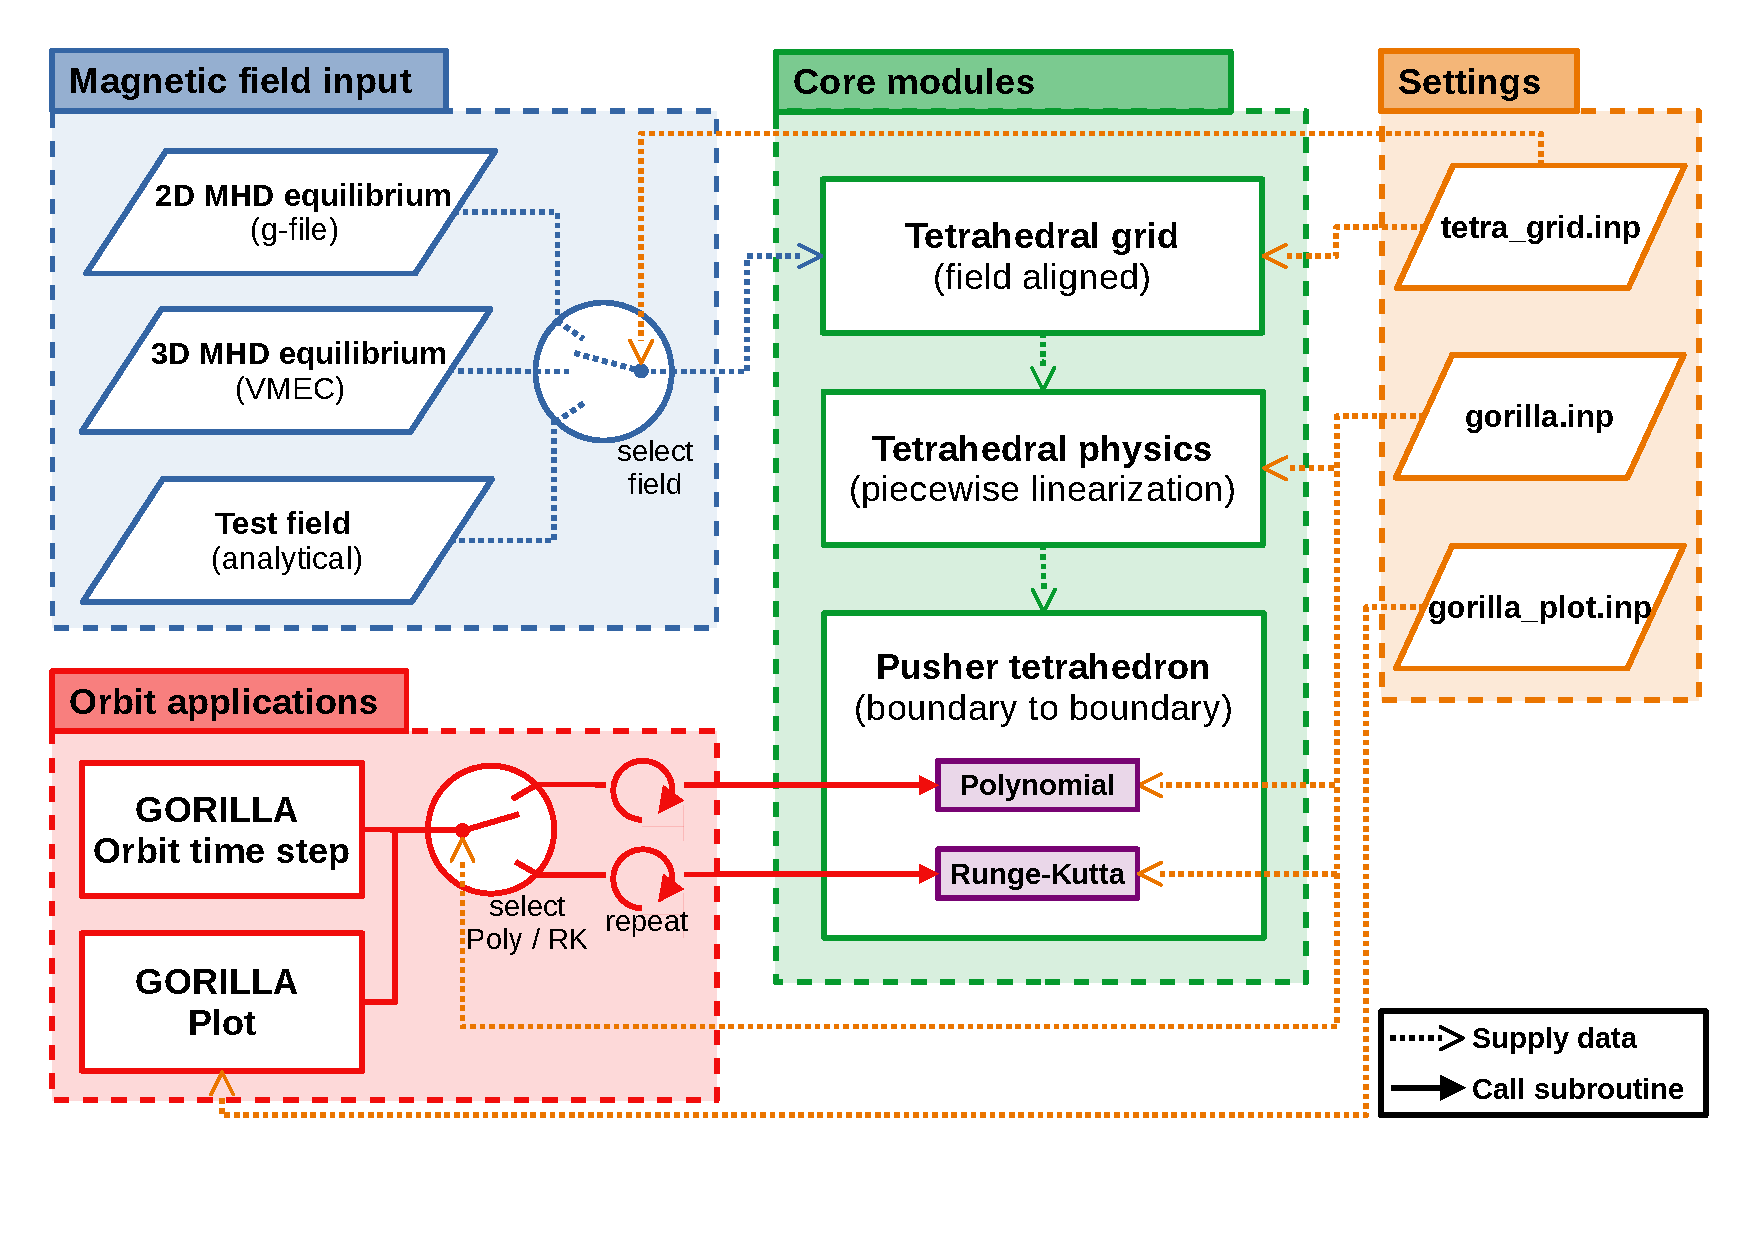
\includegraphics[keepaspectratio,width=1.05\linewidth, trim=0 50 0 20, clip]{figures/flow_diagram_GORILLA_01.pdf}}
	\captionsetup{justification=raggedright,singlelinecheck=false,textfont=footnotesize,labelfont=footnotesize}
	\caption{General overview of the structure of GORILLA: Core modules,  magnetic field input,  settings and orbit applications. Dotted lines with line-arrows indicate supply of data for subsequent execution of subroutines. Solid lines with filled arrows show the direction of subroutine calls. (Data flow of called subroutine return values is implied in the opposite direction.)}
	\label{fig:flow_diagram_GORILLA_01}
\end{figure}

For various simulations in magnetic confinement fusion, direct modeling of guiding-center particle orbits is utilized, e.g. 
global kinetic computations of quasi-steady plasma parameters or fast alpha particle loss estimation for stellarator optimization; see introduction of this thesis.
In such complex simulations a simple interface for the guiding-center orbit integration part is needed. Namely, the initial condition in five-dimensional phase space is provided (e.g. guiding-center position, parallel and perpendicular velocity) and the main interest is in the condition after a prescribed time step while the integration process itself is irrelevant. 
Such a pure ``orbit time step routine'' acting as an interface with a plasma physics simulation is provided (``\textit{GORILLA orbit time step}'').
However, in the context of this work the integration process itself is of high interest as well, thus, a program allowing the detailed analysis of guiding-center orbits, their respective invariants of motion and Poincaré plots is at disposal as well (``\textit{GORILLA Plot}''). Both orbit application routines can be used independently from each other, whereby they utilize the same underlying modules and subroutines. 
%Settings and visualization examples of \textit{GORILLA Plot} can be found in appendix~\ref{sec:gorilla_plot}.

In Fig. ~\ref{fig:flow_diagram_GORILLA_01} a general overview of the structure of GORILLA is depicted, where these two orbit application routines can be seen in a red box. 
The blue box shows the input options for the magnetic field, which can be either provided by magnetohydrodynamics (MHD) equilibria in 2D (e.g. EFIT\cite{lao_reconstruction_1985,lao_equilibrium_1990}) and in 3D (e.g. VMEC\cite{hirshman_steepestdescent_1983,hirshman_three-dimensional_1986}, GPEC\cite{park_computation_2007,logan_neoclassical_2013}) or by an analytical test field. \\
%
The major part of GORILLA can then be divided in three separate core modules, which are depicted in green. First, the \textit{tetrahedral grid module} loads the magnetic field data and generates a 3D field-aligned grid consisting of tetrahedra.  
Second, in the \textit{tetrahedral physics module} the electromagnetic field is linearly interpolated within the tetrahedra of the grid such that globally (in the plasma core) the field is represented by piecewise linear functions. Further, normal vectors describing the planes which confine the tetrahedra and which are later needed are computed.  
Third, the actual guiding-center orbit integration is performed in the \textit{pusher tetrahedron module}, where ``a particle is pushed from tetrahedral cell boundary to cell boundary, if no intermediate position inside a cell, e.g. after a pre-defined time step, is required deliberately. The positions before and after the time step are, in general, located inside the cells while the time step itself includes tracing of all orbit intersections with cell boundaries between these positions.''\cite{eder_quasi-geometric_2020} For such pushing of a particle, a numerical \textit{Runge-Kutta} and a \textit{Polynomial} option, as briefly described in Ref.~\onlinecite{eder_quasi-geometric_2020}, are implemented. These options are depicted in violet boxes. Eventually, one of the two pushing options is repeatedly called in a loop (within the orbit applications) until the prescribed time is elapsed. 

All settings for the grid generation, the orbit integration and the plotting of full orbits, Poincaré sections and the time evolution of invariants of motion are governed by the input files \texttt{tetra\_grid.inp}, \texttt{gorilla.inp} and \texttt{gorilla\_plot.inp} which are visible in orange.  E.g., a switch parameter in \texttt{gorilla.inp} determines whether the \textit{Runge-Kutta} or the \textit{Polynomial} option is used.
%

\section{Field-aligned tetrahedral grid with linearized electromagnetic field \\ quantities}
\label{sec:tetrahedral_grid}
%
In this section an overview is given how the grid which is used in GORILLA is generated. This grid consists of tetrahedral cells and is aligned to the magnetic field.  A detailed description of the grid generation (with some modifications) including also a non-field-aligned grid can be found in Ref.~\onlinecite{bauer_master_2020}. 
Furthermore, inside the tetrahedral cells the quantities describing the electromagnetic field are independently approximated by linear functions.\\



\textbf{Magnetic field input:}\\
%
As stated in section~\ref{sec:gorilla_structure}, the magnetic field must be either provided by an MHD equilibrium or by an analytical test field. As shown below, for the utilization in GORILLA a field-aligned grid has an inherent benefit with respect to the linear interpolation of the covariant component of the vector potential when this is represented in flux coordinates. Without going into details, the working principle of GORILLA requires neither flux coordinates nor a field-aligned grid. However, non-flux coordinates, e.g. cylindrical coordinates, affect the shape of guiding-center orbits significantly and can also lead to artificial chaos in the case of three-dimensional fields. These circumstances are explained and illustrated in detail in section IIIB of Ref.~\onlinecite{eder_quasi-geometric_2020}.\\
%
Without loss of generality, we use (straight field-line) symmetry flux coordinates\cite{dhaeseleer_flux_2012} $(s,\vartheta,\varphi)$ here, where $s$ denotes the flux label (normalized poloidal or toroidal flux), $\vartheta$ the symmetry flux poloidal angle and $\varphi$ the toroidal angle, respectively. A prerequisite for the generation of a field-aligned grid to be used in GORILLA is that the following quantities which represent the electromagnetic field are available as functions of arbitrary positions inside the plasma core: $A_k$, $B_k$, $\omega_c$, $\Phi$ and $\sqrt{g}$, which are the covariant components of the vector potential and the magnetic field, the cyclotron frequency, the electrostatic potential and the metric determinant, respectively. If these are not inherently available through analytic functions (in the case of a test field), interpolation of data points (in the case of MHD equilibria) and appropriate transformation to symmetry flux coordinates (SFC) are needed. Here, it should be mentioned that the divergence freeness of the magnetic field must not be violated. Since it is not an inherent part of this work, a description how to achieve such a transformation and interpolation is omitted, instead we assume that the above mentioned quantities are available as functions of SFC. A detailed description can be found in Ref.~\onlinecite{bauer_master_2020}.\\


\textbf{Requirements and structure of the tetrahedral grid:}\\
There exist several requirements that must hold for a tetrahedral grid in order to function correctly while being used in GORILLA. ``These requirements are: 

\begin{enumerate}
	\item The three-dimensional spatial domain, which is relevant for calculations, must be fully covered by non-overlapping tetrahedra. In this application tetrahedra are necessary since field quantities are used in a piecewise linearized form, meaning they are saved as a scalar value at a reference point and a corresponding gradient of the quantity. Such a linear representation has four independent parameters, therefore, the use of tetrahedra is ideal since the parameters of the linearized field quantity can be exactly defined via the field quantities at the four vertices of the tetrahedron. One might think that apart from tetrahedra other spatial objects with more vertices can still be used by fitting a linear function of the field quantity, however, such an application would destroy the important property that the field quantities through adjacent faces of tetrahedra are continuous.
	Furthermore, for vector quantities each vector component is independently linearized.
	
	
	\item All edges of tetrahedra must coincide with edges of neighboring tetrahedra. Edges that lie on faces of neighboring tetrahedra (these are called \textit{hanging nodes}) or crossings between edges are not permitted. This requirement is given by the continuity condition of linearized field quantities through the faces of each tetrahedron.
	
	\item Each tetrahedron must be defined via four corner vertices in a given coordinate system. The coordinate values of each vertex are stored in an array and each vertex is identified by its array index. The index of the four vertices belonging to a specific tetrahedron has to be stored in a $4\times1$ array and can be accessed by indices 1 to 4 within each tetrahedron.
	
	\item The tetrahedra are stored in an array of tetrahedron objects and identified by their index. Each tetrahedron has four defined faces labeled face 1 to 4. Each face $i$ ($i = 1,2,3,4$) is spanned by the vertices of the tetrahedron excluding tetrahedron-vertex $i$. For instance, face 3 will be spanned by tetrahedron-vertices 1,2,4. This implies that the tetrahedron-vertex $i$ will be the only tetrahedron-vertex not lying on face $i$.
	
	\item For a given tetrahedron, the neighboring tetrahedron which is separated by the $i$-th face of the current tetrahedron will be considered the neighbor $i$ to the current tetrahedron with its global labeling index being saved in the $i$-th position of a $4\times1$ array.
	
	\item In addition to saving the four faces and neighbors of each tetrahedron, the index of the intersecting face between the original tetrahedron and its neighbor in the index system of the neighbor will be saved with the original tetrahedron. This means that the face through which a particle enters a neighbouring tetrahedron can be determined by knowing through which face it is leaving the current one.
	
	\item Tetrahedra at the outer boundary of the grid will not have neighboring tetrahedra at the boundary face, the neighboring tetrahedron index as well as the index of the face in the index system of the neighboring tetrahedron will be set to $-1$.
	
	\item The normal vectors corresponding to each face of all tetrahedra must be explicitly calculated and saved together with a reference point. This enables the calculation of normal distances of any arbitrary point to all faces of each tetrahedron.
	
	\item Grids that are made in a coordinate system with a periodic coordinate need to have an additional property set for tetrahedra faces lying at the periodic boundary, depending on which side the face lies. This determines in which direction the coordinate needs to be shifted when the particle passes through the boundary.''\cite{bauer_master_2020} In the case that an approach with Cartesian coordinates is used for the particle position exchange in-between adjacent tetrahedral cells, see section~\ref{ssec:auxiliary_methods}, this requirement can be neglected.
	
	\item In the case of axisymmetry of the electromagnetic field (with respect to the toroidal direction, e.g. field inside a tokamak),  this symmetry property must not be violated when approximating field quantities with piecewise linear functions.\\
\end{enumerate}



\textbf{Generation of the vertices of the tetrahedral grid:}\\
``The first step in implementing this grid is to generate the vertices that will define the corner points for the tetrahedral cells filling a given space. In order to achieve this, the domain which will be covered by the grid needs to be specified in the coordinate system where the grid will be generated.''\cite{bauer_master_2020} In this case, we choose SFC as described above. In its most simple form, the grid will have vertices equidistantly spaced in $s,\vartheta$ and $\varphi$ direction with intervals for $s$ being $[0,1]$, $[0,2\pi]$ for $\vartheta$ and $[0,2\pi/N_\text{fp}]$ for $\varphi$, where $N_\text{fp}$ is the number of field periods of the toroidal fusion device. \\
%
``Now, each coordinate $x_i$ will be discretized into $N_i$ equidistant values for each given interval. Using nested loops, these discretized values will be connected to $N_s\times N_\vartheta \times N_\varphi$ unique triples representing the coordinates of the individual vertices of the grid.''\cite{bauer_master_2020} As a result, one obtains the vertices of a regular grid consisting of hexahedra, if all vertices are connected to their nearest neighbors, assuming that all intervals are normalized to the same value. These hexahedral cells are subsequently split into tetrahedral cells as shown below.\\
%
The coarseness of the hexahedral grid, which also implies the total number of tetrahedral cells, is defined by $N_i$. Thus, we call $N_s\times N_\vartheta \times N_\varphi$ the ``grid size'' of the tetrahedral grid. However, in order to obtain the number of tetrahedral cells the product of this grid size must be multiplied by the number of tetrahedral cells per hexahedron.\\



\textbf{Generation of tetrahedral cells and linearized electromagnetic field quantities:}

\begin{figure}[h]
	\centerline{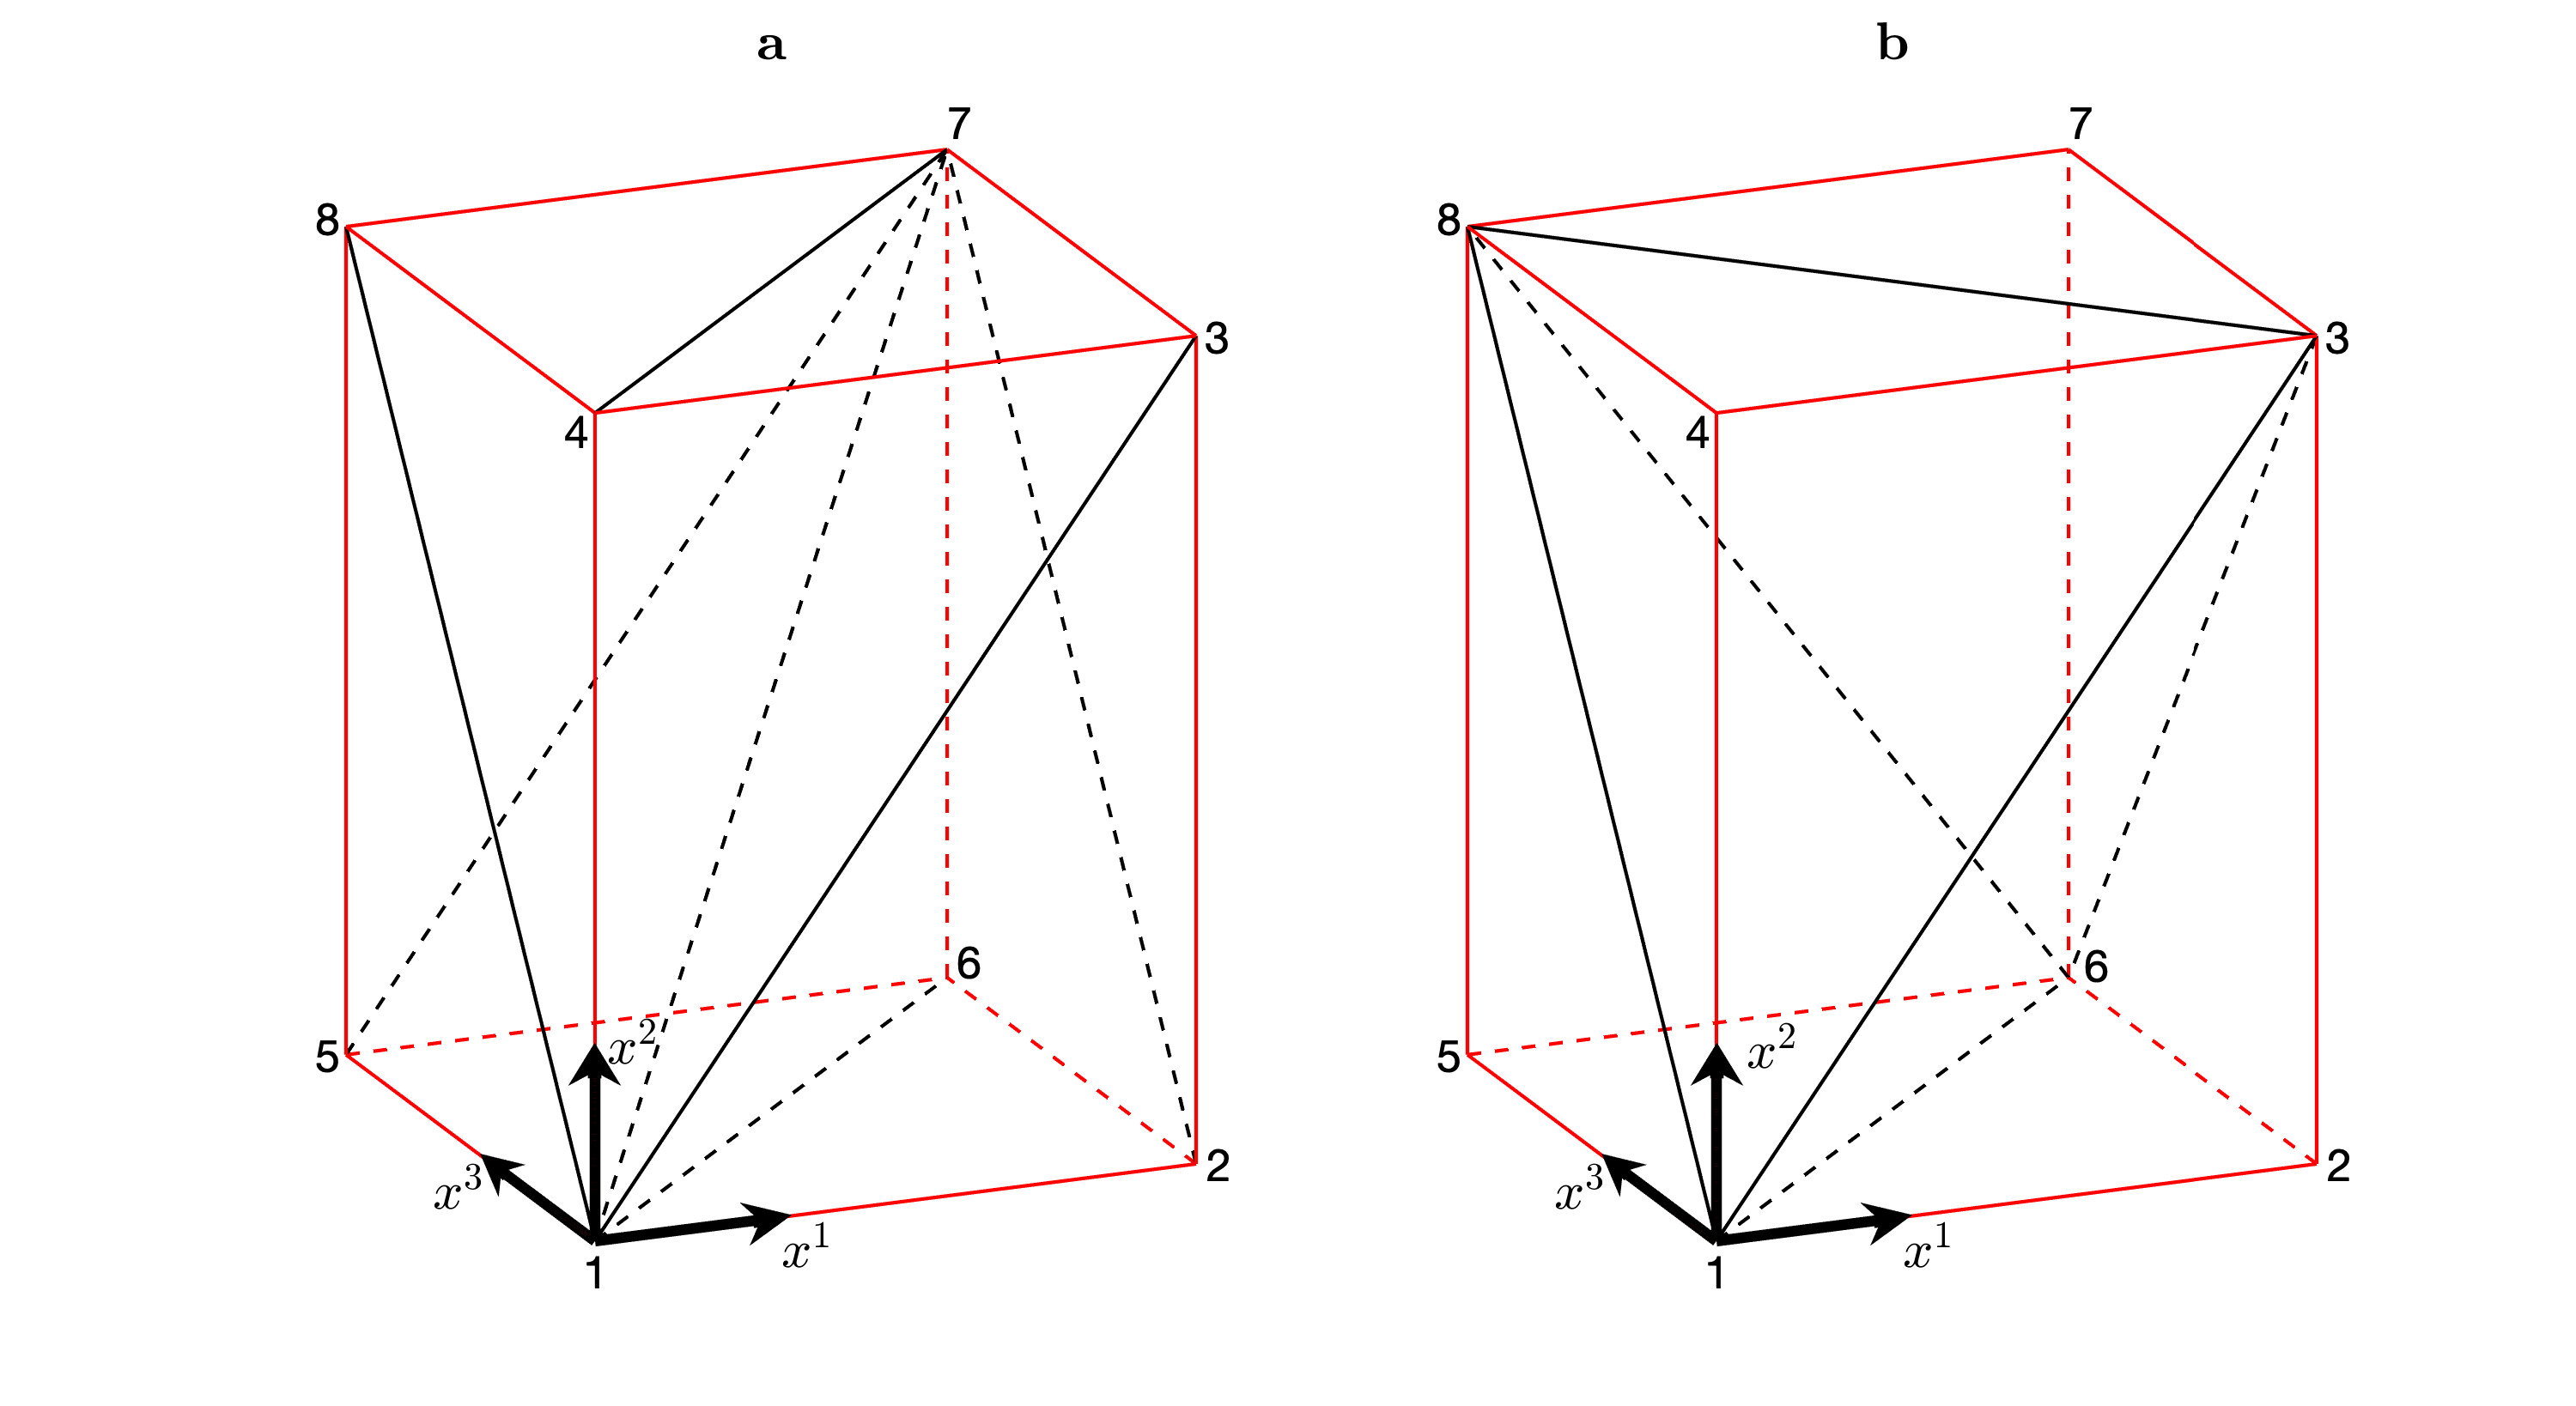
\includegraphics[keepaspectratio,width=1.05\linewidth, trim=120 50 100 5, clip]{figures/tetraeder.eps}}
	\captionsetup{justification=raggedright,singlelinecheck=false,textfont=footnotesize,labelfont=footnotesize}
	\caption{Flux coordinate space illustration of two realizations of a hexahedron (red) being split into tetrahedral cells. The symmetry direction is along the coordinate $x^3$.\\
	(a) The hexahedron is split into six tetrahedral cells such that the axisymmetry property of the electromagnetic field is preserved upon linearization of field quantities.\\
	(b) The hexahedron is split into five tetrahedral cells without preserving axisymmetry upon linearization.}
	\label{fig:splitting_hexahedra}
\end{figure}

As stated in section IIA of Ref.~\onlinecite{eder_quasi-geometric_2020}, the field quantities $A_k$, $B_k/\omega_c$, $\omega_c$ and $\Phi$ are independently approximated by continuous piecewise linear functions. This approximation is achieved by linearly interpolating the field quantities inside the tetrahedral cells of the described grid. Here, it should be mentioned that the exact field values are retained on the tetrahedral cell's vertices. \\
%
In the case that the electromagnetic field is axisymmetric with respect to the toroidal direction, this symmetry property must not be violated by the interpolation. Thus, the tetrahedral cells must be specially oriented in order to preserve this symmetry and its respective invariant of motion of the guiding-center equations; see section IIA of Ref.~\onlinecite{eder_quasi-geometric_2020}.
``Namely, this is achieved with stackable hexahedra each consisting of two triangular prisms which are both subsequently split into
3 tetrahedral cells.  The prisms are oriented such that all triangular prism faces lie on
$x^3= \mathrm{const.}$ planes where $x^3$ is the symmetry direction.
Thus, each tetrahedron face which lies on a $x^3= \mathrm{const.}$ plane is congruent with
all other tetrahedron faces opposing it in the symmetry direction.''\cite{eder_quasi-geometric_2020}
This specific splitting realization can be seen in a real space illustration of the field-aligned grid in Fig. 1 of Ref.~\onlinecite{eder_quasi-geometric_2020}. Furthermore, Fig.~\ref{fig:splitting_hexahedra} (a) shows this specific splitting realization which is used in GORILLA in flux coordinate space. For a better understanding of the preservation of axisymmetry, let us assume that the modulus of the magnetic field $B$, which is proportional to the cyclotron frequency, $\omega_c = e B / m c$, is exactly given on the 8 vertices of the hexahedron in Fig.~\ref{fig:splitting_hexahedra} (a). In an axisymmetric field, the respective values at vertices which oppose in the symmetry direction $x^3$ remain constant, e.g.  $B$ has the same value at vertex $1$ and $5$. Due to the linearization, the value of $B$ at a random position $(x^1_a,x^2_a,x^3_a)$ on the triangular tetrahedron face confined by the vertices $1,2$ and $3$ is a linear superposition of the values of $B$ at these vertices. If we keep $x^1_a,x^2_a$ constant and make a variation of the component $x^3_a$, the point describing the position will cross the tetrahedral cell boundary and eventually reach the triangular tetrahedron face confined by the vertices $5,6$ and $7$. Throughout this variation, the value of $B(x^1_a,x^2_a,x^3_a)$ remains constant, since the values at the vertices opposing in the symmetry direction remain constant, while the vertices themselves, which are the basis of the superposition, change when entering an adjacent tetrahedron.\\
%
In contrast, Fig.~\ref{fig:splitting_hexahedra} (b) shows an alternative splitting realization, where the field property of axisymmetry is not preserved. The triangular tetrahedron face confined by the vertices $1,2$ and $3$ is not opposed by a congruent triangular face in the symmetry direction. E.g., the value of $B$ at a random position $(x^1_b,x^2_b,x^3_b)$ on the triangular face with the vertices $1,2$ and $3$ is in general affected by the value at vertex $3$, while the non-congruent opposing triangular face with the vertices $5,6$ and $8$ has the same $B$ values at vertices $5$ and $6$ but not at vertex $8$. If we make the same variation as above, namely keeping $x^1_b,x^2_b$ constant and change only $x^3_b$, the value of $B(x^1_b,x^2_b,x^3_b)$ will in general change throughout this variation.\\
%
Moreover, if one carefully observes the splitting realization of Fig.~\ref{fig:splitting_hexahedra} (a), one can see that symmetry is not only preserved in the $x^3$ direction, but that the criterion for conservation (upon linearization) is also valid for the directions $x^1,x^2$ in the case that these directions posses a symmetry property.  In particular, in the case of transport optimized stellarators\cite{mynick_transport_2006} a grid with this specific splitting realization should preserve the quasi-axisymmetry ($B$ is independent of the toroidal angle $\varphi$) and quasi-poloidal symmetry ($B$ is independent of the poloidal angle $\vartheta$). \\
%
Finally,  for the utilization in GORILLA a field-aligned grid has an inherent benefit with respect to the linear interpolation of the covariant component of the vector potential $A_k$ when this is represented in flux coordinates.
With the appropriate gauge transformation, $A_k$ can be denoted in SFC as $A_s = 0$, $A_\vartheta = s \psi_\text{tor}^\text{max}$ and $A_\varphi= \psi_\text{pol}$, where $s$, $\psi_\text{tor}^\text{max}$ and $\psi_\text{pol}$ are the normalized toroidal flux surface label, the toroidal flux at the separatrix and the poloidal flux, respectively.
In the described linearization approach, for vector quantities each vector component is independently linearized. Thus, with this representation of $A_k$ in SFC, no interpolation errors in the poloidal and toroidal direction are introduced, since none of the covariant components of $A_k$ are dependent on $\vartheta$ or $\varphi$. As a consequence, the existence of flux surfaces is not violated in piecewise linear toroidal fields. However, due to the s-dependence of $\psi_\text{pol}$, the rotational transform, $\iota = \psi^\prime_\text{pol} /  \psi^\prime_\text{tor}$, is a piecewise constant function in this approach. Associated consequences with respect to artificial chaotization are discussed in detail in section IIIB of Ref.~\onlinecite{eder_quasi-geometric_2020}.\\


\textbf{Numerical implementation:}\\
In the numerical implementation of GORILLA, the \textit{tetrahedral grid module} loads the magnetic field data and generates the field-aligned tetrahedral grid with the (symmetry preserving) splitting procedure of a regular hexahedral grid in flux coordinate space. Further, the linear interpolation of the electromagnetic field quantities is performed within the \textit{tetrahedral physics module} as well as the construction of normal vectors who describe planes which confine these tetrahedra and which are essentially needed in the subroutines for appropriately pushing particles through the tetrahedral cells; see below.\\
%
The technical details of the remaining implementation of a logic that fulfils the requirements from above, namely the indexing of tetrahedra, their faces and the indexing of the respective neighboring tetrahedra and their adjacent faces, etc., are omitted in this work, since this chapter is intended to present the code in a concise and unified manner.  A detailed description can be found in Ref.~\onlinecite{bauer_master_2020}.

\section{Algorithm for pushing particles \\ through tetrahedral cells}
%
\begin{figure}[h]
	\centerline{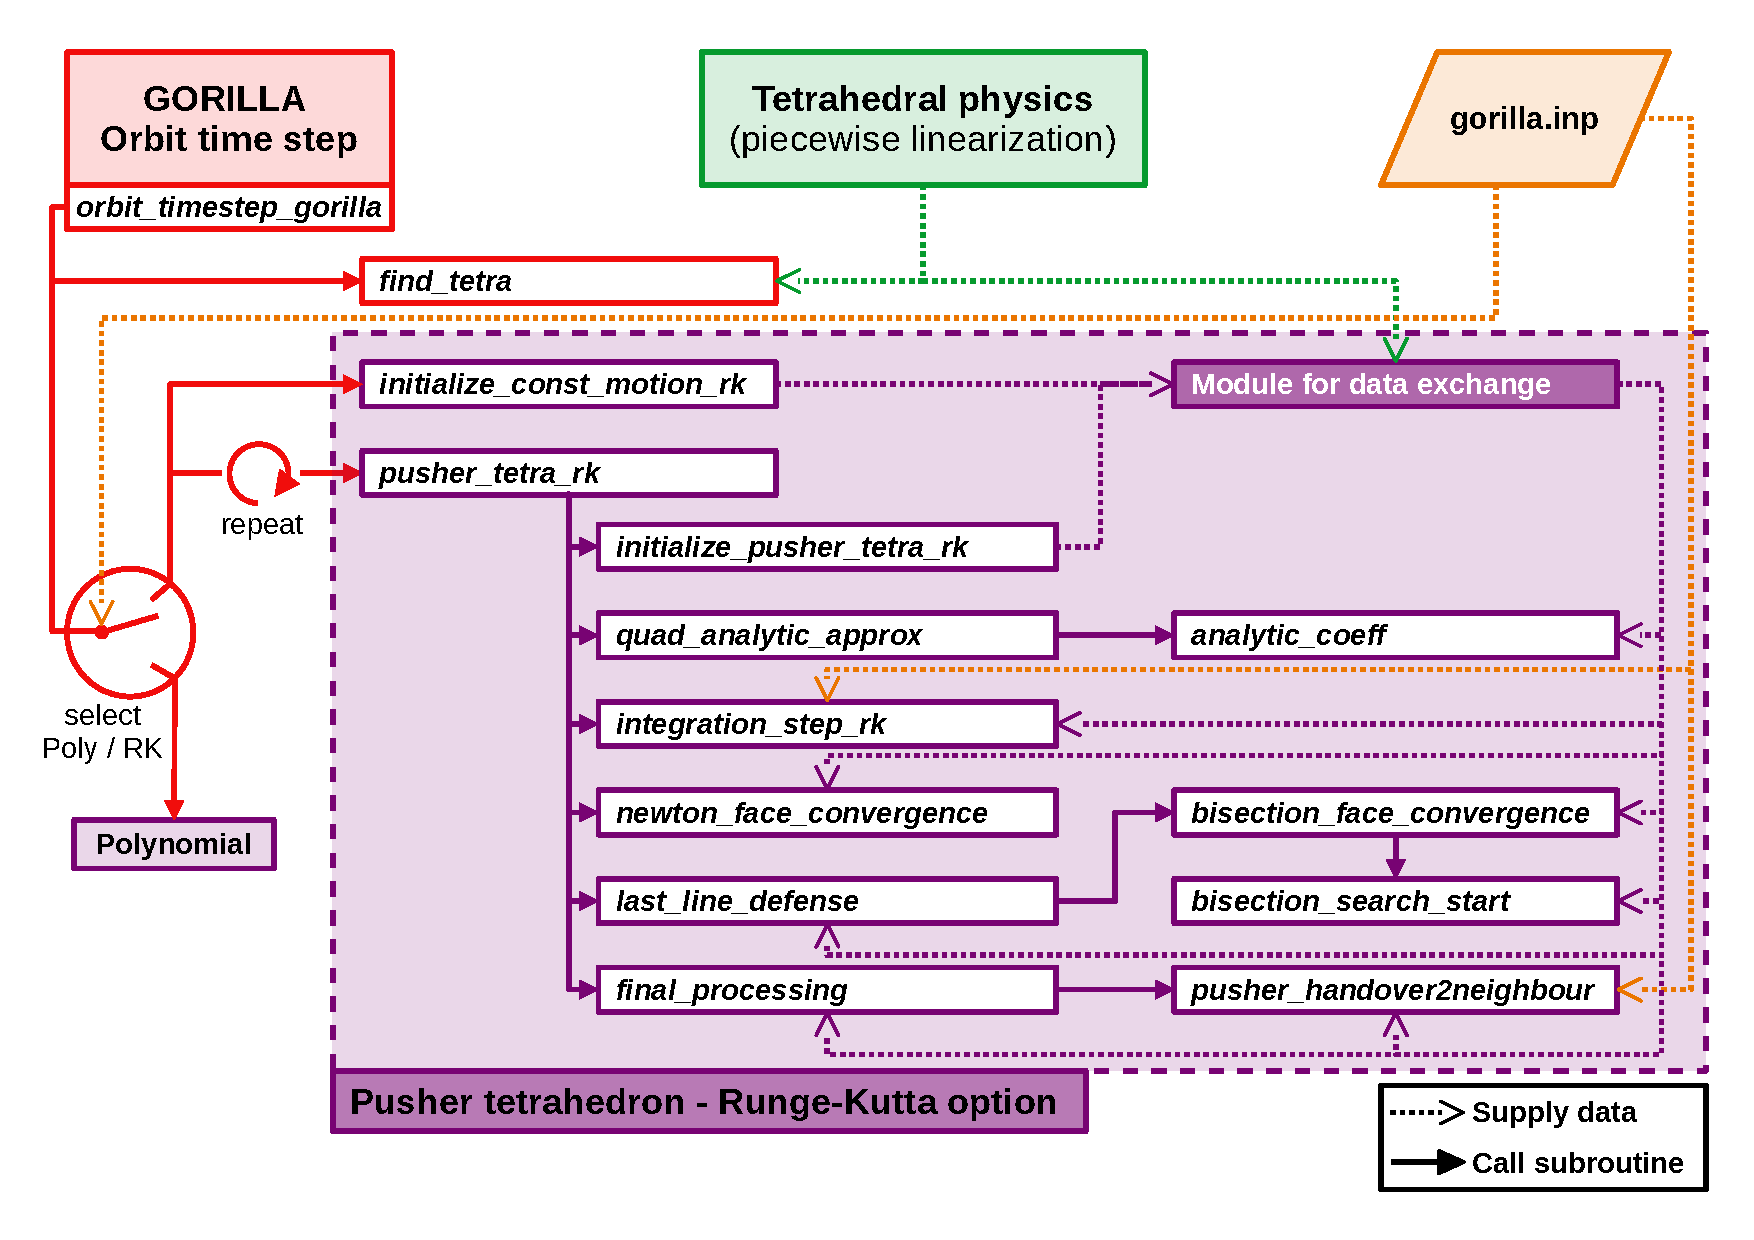
\includegraphics[keepaspectratio,width=1.05\linewidth, trim=0 20 0 20, clip]{figures/flow_diagram_GORILLA_03.pdf}}
	\captionsetup{justification=raggedright,singlelinecheck=false,textfont=footnotesize,labelfont=footnotesize}
	\caption{Overview of the structure of the \textit{Runge-Kutta option} belonging to the \textit{pusher tetrahedron module} of GORILLA. Dotted lines with line-arrows indicate supply of data for subsequent execution of subroutines. Solid lines with filled arrows show the direction of subroutine calls. (Data flow of called subroutine return values is implied in the opposite direction.) \textit{This figure is taken from Ref.~\onlinecite{bauer_master_2020} and modified.}}
	\label{fig:flow_diagram_GORILLA_03}
\end{figure}
%
In this section an overview of the algorithm to integrate a guiding-center orbit by consecutively pushing a particle through tetrahedral cells (with its two options \textit{Runge-Kutta} and \textit{Polynomial}) is presented. As can be seen in Fig.~\ref{fig:flow_diagram_GORILLA_01}, this is done within the \textit{pusher tetrahedron module}. The working principle of the required routines and auxiliary methods is briefly explained.  Without loss of generality, here, we limit to only one orbit application, namely \textit{GORILLA orbit time step.} The second orbit application (\textit{GORILLA Plot}), which is intended for the analysis of the quasi-geometric integration method itself, is working in the same manner with some additional diagnostic extensions intended for visualization.

``The focus of the \textit{pusher tetrahedron module} lies, however, not only on the computation of the trajectory and the calculation of the next tetrahedron intersection but rather on finding a numerically inexpensive scheme that allows to save computational cost while reliably yielding accurate results for the intersection of the orbit with the tetrahedron. While the results are in theory equivalent for both pushing options, the approaches are completely independent and thus may vary in both computational efficiency and numerical accuracy, depending on up to which polynomial order $K$ of Eq.~(11) of Ref.~\onlinecite{eder_quasi-geometric_2020} the orbit is computed.''\cite{bauer_master_2020} \\
%
Due to the interchangeability of these two options, we will demonstrate the common algorithmic approach, now, by only referencing to the \textit{Runge-Kutta option}. The distinctive details of these two options are subsequently discussed in separate sections. \\
%
Fig.~\ref{fig:flow_diagram_GORILLA_03} shows the overview of the structure of the \textit{Runge-Kutta option}, belonging to the \textit{pusher tetrahedron module} of GORILLA, and, as well, how this module is called from the orbit application \textit{GORILLA orbit time step.} The actual \textit{Runge-Kutta option} is depicted in a violet box. \\
%
A prerequisite for the functionality of this module is the pre-computed linearized electromagnetic field, as well as the normal vectors describing the planes which confine the tetrahedra. Both are provided by the \textit{tetrahedral physics module} (green in Fig.~\ref{fig:flow_diagram_GORILLA_03}). All necessary settings including the pushing option (\textit{Runge-Kutta} or \textit{Polynomial}) are governed by the input file (orange in Fig.~\ref{fig:flow_diagram_GORILLA_03}).\\
%
The \textit{GORILLA orbit time step} application is realized as a wrapping routine with the name \texttt{orbit\_timestep\_gorilla} (red in Fig.~\ref{fig:flow_diagram_GORILLA_03}) which is given the initial conditions of the particle and returns the condition after the pre-defined time step.\\
%
``For starting a particle at a given position without knowing to which tetrahedron it belongs to in coordinate space, an auxiliary routine \texttt{find\_tetra} was constructed for efficiently finding the corresponding tetrahedron index to start a calculation''\cite{bauer_master_2020}; see section \ref{ssec:auxiliary_methods}.  This routine must be called only at the very first time when a particle is started.  Further subsequent orbit time steps, e.g.  after a scattering process in a simulation, do not require to find the appropriate tetrahedron in the grid anymore, as long as the particle position stays unchanged in-between consecutive time steps, and thus, the information to which tetrahedron the particle belongs can be retained.\\
%
The first subroutine to be called for an orbit time step within the \textit{pusher tetrahedron module} (and after the appropriate tetrahedron has been found) is \linebreak \texttt{initialize\_const\_motion\_rk} which sets the constants of motion (perpendicular adiabatic invariant $J_\perp$ and respective squared value) for the given initial conditions.
``The constants of motion will retain their set values for a number of tetrahedral pushings until the next time step is executed. Usually, in-between time steps collision events will occur. As a consequence, the constants of motion may change and have to be defined anew for every orbit time step.''\cite{bauer_master_2020} \\
%
Eventually,  the subroutine \texttt{pusher\_tetra\_rk} which is responsible for the actual pushing through a tetrahedral cell is called repeatedly inside the wrapping routine until the pre-defined time is elapsed.  Since, in general, the pre-defined time step for an orbit will lead to a particle position somewhere inside a final tetrahedron, the remaining time of the orbit to reach the pre-defined time must be given to the subroutine \texttt{pusher\_tetra\_rk} when being called repeatedly. ``This subroutine then computes the time it takes until the particle exits the current tetrahedron and compares this value to the remaining time of the orbit time step.  In the case the time it takes to leave the tetrahedron is smaller than the remaining time of the orbit time step, the pushing is computed. Then, the remaining time is reduced by this value and the next pushing through the adjacent tetrahedron is started. In the case there is not sufficient time to complete the pushing, the orbit is instead integrated up to the value of the orbit parameter $\tau$ corresponding to the remaining time, leading to a final position somewhere inside the tetrahedron.''\cite{bauer_master_2020}\\
%
The strategy how to achieve a pushing through a tetrahedral cell with the \textit{Runge-Kutta} option (within the subroutine \texttt{pusher\_tetra\_rk}) and, specifically, in a computationally efficient manner is discussed in the following. The algorithm for the \textit{Polynomial} option is identical until here, apart from calling the subroutines \texttt{initialize\_const\_} \texttt{motion\_poly} and \texttt{pusher\_tetra\_poly} instead.  The latter subroutine realizing the alternative polynomial approach is discussed below as well.
%
\subsection{Numerical approach with Runge-Kutta}
\label{ssec:gorilla_runge_kutta}
%
The subroutine \texttt{pusher\_tetra\_rk} is called with the initial conditions of the particle, namely position and parallel and perpendicular velocity, as well as the required tetrahedron information, namely the indices of the appropriate tetrahedron and tetrahedron face. The face index takes the values $1 \dots 4$, meaning that the particle's position lies in on one of the four tetrahedra faces, or $0$ in the case the particle's position is somewhere inside the tetrahedron.  In addition, also the remaining time of the orbit time step prior the pushing is given to \texttt{pusher\_tetra\_rk}.  In the violet box in Fig.~\ref{fig:flow_diagram_GORILLA_03} one can see the subroutines used within the \textit{Runge-Kutta option} for pushing a particle through a tetrahedron.
After the execution, the subroutine returns the new initial conditions for a subsequent pushing through a tetrahedron, as well as the remaining time of the orbit time step after the pushing. \\
%

\textbf{Initialize the module for data exchange:} \\
``In the \texttt{pusher\_tetra\_rk} subroutine, first an initialization subroutine \texttt{initialize\_pu} \texttt{sher\_tetra\_rk} is called. Here, the initial conditions are used to compute the coefficients $a^i_l, b^i$ for the ordinary differential equation set~(5) of Ref.~\onlinecite{eder_quasi-geometric_2020} representing the equations of motion in the specific tetrahedron. One should emphasize here, that this ODE set is solved within a shifted coordinate system, where the coordinate origin lies on the first vertex of the given tetrahedron.''\cite{bauer_master_2020}\\

\textbf{Initial guess of exit time and exit face:}\\
Now, the intersection between the orbit and the tetrahedral cell which can be reached in the smallest positive time from the initial position (``exit time'') and its appropriate tetrahedral face (``exit face'') needs to be computed. (A representative illustration can be seen in Fig.~2 of Ref.~\onlinecite{eder_quasi-geometric_2020}.) ``Since this must be done efficiently, a numerically inexpensive approximative quadratic solution is first evaluated by subroutine \texttt{quad\_analytic\_approx} to compute the guess for the orbit parameter $\tau$ at the first intersection of the particle trajectory with the cell boundary. Based on the approximative (quadratic) result for the orbit parameter $\tau$, an integration step is performed for the given step length''\cite{bauer_master_2020} using \texttt{integration\_step\_rk}. This subroutine solves the initial value problem for the set~(5) of Ref.~\onlinecite{eder_quasi-geometric_2020} either, determined by the user, with a single step of the Runge-Kutta 4 method (RK4) or with the adaptive Runge-Kutta 4/5 method (RK4/5) and returns the evaluated position. \\
%
``In general, due to inaccuracies in the approximation, this value does not correspond to a ``converged'' orbit position. In the context of the subroutine \texttt{pusher\_tetra\_rk}, converged simply means that the particle position is within a defined convergence distance to a given tetrahedral plane. This distance can be set manually. Its default value is $10^{-10}$ times the normal distance of the first vertex within a given tetrahedron to its opposing cell boundary spanned by vertices 2,3 and 4 of the given tetrahedron. In addition, the normal velocity, which can also be computed from the output of the RK integration step, must have a negative sign in order for the convergence to be valid.''\cite{bauer_master_2020} (By definition, the normal vectors describing the planes which confine the tetrahedra are pointing inwards.) ``The negative sign assures here, that only outflowing particles (i.e. with negative normal velocity) are accepted as a solution.  
Now, since the orbit position is generally not yet converged after the quadratic approximation, one next applies Newton's method for the convergence of the orbit position on the tetrahedron face by calling the subroutine \texttt{newton\_face\_convergence}.''\cite{bauer_master_2020} There, Runge-Kutta integration steps are embedded into an iterative scheme using Newton’s method in various orders. A detailed description of this approach is given in Ref.~\onlinecite{eder_master_2018}.\\

\textbf{Convergence and validation loop (\texttt{conv\_val\_loop}):}\\
``What one has obtained so far is a proposal for the exit plane and a converged orbit position on this plane. There may still be some problems, however, since for example Newton's method can fail if the orbit in fact turns before it intersects with the plane. Furthermore, it might happen that it does converge on the suggested plane but at the point of convergence it had already left the tetrahedron through another plane which is not allowed as it would be the actually correct exit plane instead of the proposed one. Such cases need to be checked and handled appropriately. For this purpose, the \textit{convergence and validation loop} (\texttt{conv\_val\_loop}) was implemented. This loop starts directly after the above mentioned quadratic approximation just before the convergence using Newton's method. Here, in each iteration of the loop, the algorithm tries to converge the particle orbit position on the currently proposed intersection face. Next, if convergence is reached the algorithm checks for the remaining planes if the particle lies outside the tetrahedron. If this is not the case, furthermore, the normal velocity is checked to see if the particle flies outside. In case this is also correct, the particle is considered ``converged'' and, hence, accepted. \\
%
In any case, where an error is detected, an appropriate approach is suggested. In most cases this involves using the quadratic approximation to suggest a different face, however, in some special cases this is not sufficient. Therefore, one calls inside \texttt{conv\_val\_loop} an additional convergence routine \texttt{last\_line\_defense}, which no longer opts for high computational efficiency but rather for a reliable way of finding the intersection point. \\
%
This subroutine is very comprehensive, but a central piece of it is a bisection scheme. For a short overview, in this scheme (\texttt{bisection\_face\_convergence}) one computes the relative particle positions to all four faces and furthermore checks the normal velocities. Here, if the particle is inside the tetrahedron, the current step length is doubled and an integration step is performed. If the particle is now outside the tetrahedron, the last integration step is halved and integrated back in negative $\tau$-direction. This is done in an iterative scheme until a converged particle position has been found.''\cite{bauer_master_2020} In extremely rare cases (less than one in 100 million pushings) an unsuitable starting position for the bisection procedure can lead to failure with respect to face convergence.  In such a case, the orbit is stepwise integrated in the subroutine \texttt{bisection\_search\_start} in order to find an appropriate starting position for the consecutive bisection procedure, leading to face convergence.\\
%
``Albeit the subroutine \texttt{last\_line\_defense} is computationally expensive, it remains an indispensable element of the algorithm due to its high reliability. This effect on performance remains small, however, as only a small portion of particle pushings actually need to be solved by \texttt{last\_line\_defense}.\\
%
Due to the used approach of guessing the exit face with an approximation instead of computing all intersections with all four planes, which would be computationally much more expensive, many special cases of particle trajectories had to be taken into account such that the logic deals with them correctly.''\cite{bauer_master_2020}
It should be mentioned that a lot of thought has gone into developing such an efficient and reliable logic.\\


\textbf{Final processing:}\\
Eventually, the last steps of the orbit integration are to first check if the computed time is in fact smaller than the remaining time of the orbit time step.  When this is true, the remaining time of the orbit time step which was given to \texttt{pusher\_tetra\_rk} is reduced by the exit time computed in this pushing. By calling the subroutine  \texttt{pusher\_handover2neighbour}, the tetrahedron and face index of the tetrahedron which is adjacent to the exit face will be evaluated. Due to periodic boundaries of adjacent tetrahedra, particle positions might be updated in \texttt{pusher\_handover2neighbour} which is explained in section \ref{ssec:auxiliary_methods}.  Finally, the orbit condition (position and velocities) and the tetrahedron information for the subsequent pushing are returned to the orbit application, i.e. \texttt{orbit\_timestep\_gorilla}.\\
%
If the computed time is in fact larger than the remaining time of the orbit time step, instead of the converged orbit position, the corresponding position at the remaining time is evaluated. In this case the current tetrahedron index will be returned while the face index is manually set to $0$, meaning that the particles is somewhere inside the tetrahedron.\\

\subsection{Analytical approach with polynomials}
%
\begin{figure}[h]
	\centerline{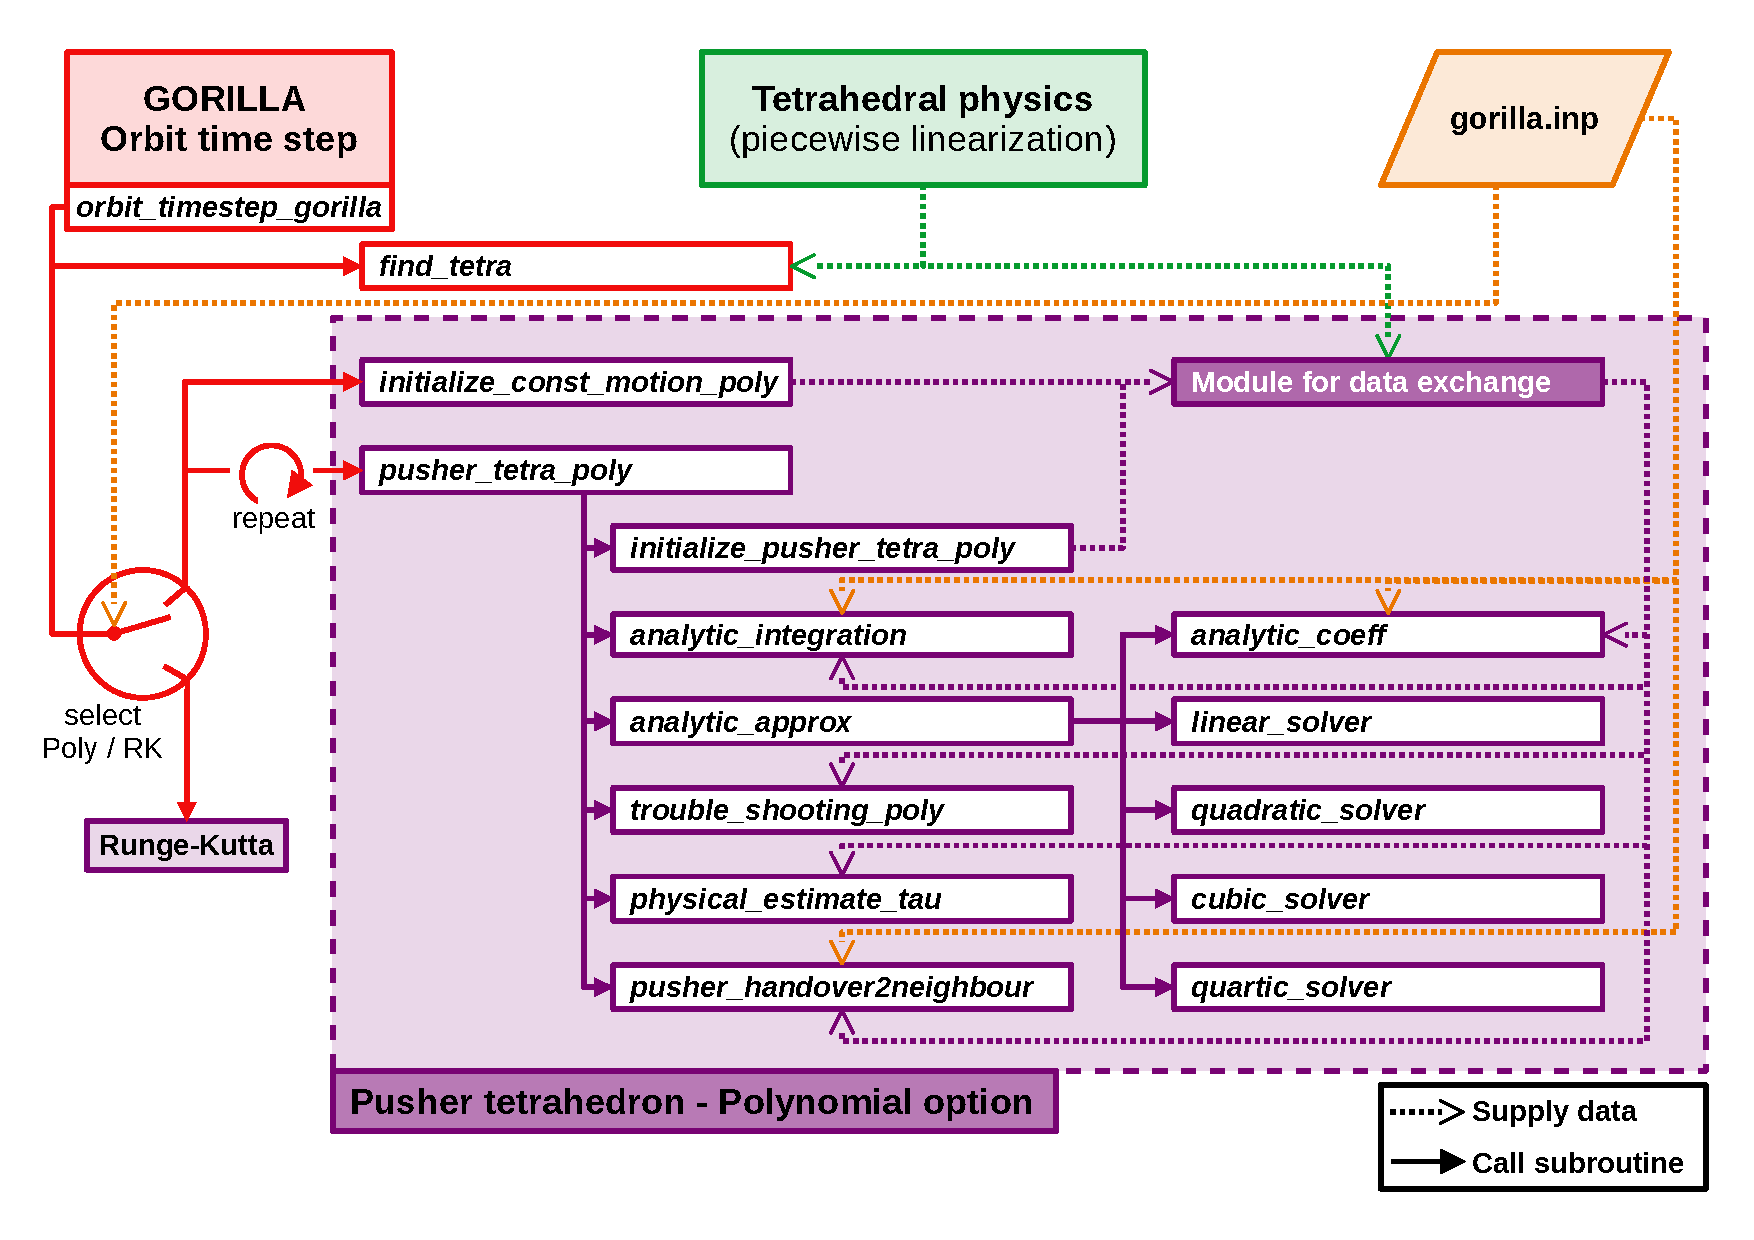
\includegraphics[keepaspectratio,width=1.05\linewidth, trim=0 20 0 20, clip]{figures/flow_diagram_GORILLA_02.pdf}}
	\captionsetup{justification=raggedright,singlelinecheck=false,textfont=footnotesize,labelfont=footnotesize}
	\caption{Overview of the structure of the \textit{Polynomial option} belonging to the \textit{pusher tetrahedron module} of GORILLA. Dotted lines with line-arrows indicate supply of data for subsequent execution of subroutines. Solid lines with filled arrows show the direction of subroutine calls. (Data flow of called subroutine return values is implied in the opposite direction.)}
	\label{fig:flow_diagram_GORILLA_02}
\end{figure}

The subroutine \texttt{pusher\_tetra\_poly} is called in the same manner as its counterpart \texttt{pusher\_tetra\_rk}, namely with the initial conditions of the particle,  as well as the required tetrahedron information and the remaining time of the orbit time step.  After the execution, the subroutine returns the new initial conditions for a subsequent pushing through an (adjacent) tetrahedron, as well as the remaining time of the orbit time step after the pushing. In the following, an overview of the working principle of the analytical approach with polynomials, which differs significantly from the numerical approach with Runge-Kutta and Newton's method, is given. \\
%
By truncating the summation of the formal solution of the locally linear guiding-center equations~(11) of Ref.~\onlinecite{eder_quasi-geometric_2020} at $K$~=~2, 3~or~4, one obtains
approximate solutions of various orders in Larmor radius. With these solutions, the equations for the exit time, which is the time it takes for the particle to reach the tetrahedral cell boundary, are algebraic equations. Thus, we call this approach ``analytical''.\\
%
In general, the orbit can be computed separately for all orders $K$~=~2, 3~or~4, however, since also in this approach computational efficiency is aspired, similarly to the RK-approach, the quadratic polynomial solution $K = 2$ is used to predict the exit face, in the case the orbit is computed with the orders $K$~=~3~or~4. This predominantly reduces the number of higher order root finding operations from four to one, while demanding an algorithm that guarantees that the ``correct'' face is found. In the context of the subroutine \texttt{pusher\_tetra\_poly}, correct simply means that the particle position is within a negligible convergence distance to the plane, which requires an accurate polynomial root finding procedure, and that the particle flies outwards the tetrahedron with respect to the exit plane.\\
%
In the violet box in Fig.~\ref{fig:flow_diagram_GORILLA_02} one can see the subroutines used within this \textit{Polynomial option}. Similarly as in the \textit{Runge-Kutta option}, by calling the initialization subroutine \texttt{initialize\_pusher\_tetra\_poly} the initial conditions for orbit integration within the specific tetrahedron are preprocessed, e.g. local coordinates, while the coordinate handling for subsequent pushing in an adjacent tetrahedron is performed within \texttt{pusher\_handover2neighbour} at the end of the pushing procedure.\\
%
For the actual orbit integration let us recall, as stated in Eq.~(14) of Ref.~\onlinecite{eder_quasi-geometric_2020} that for computing the appropriate exit time, we need to find the
smallest positive root of
\be{}
\bn^\alpha \cdot \left( \bz_0 + \sum\limits_{k=1}^K
\frac{\tau_{\red{e}\blue{d}}^k}{k!} \left(\hat \ba^{k-1}\cdot\bb + \hat \ba^k\cdot \bz_0\right)
-\bz^\alpha
\right) = 0 \quad \text{with} \quad K = 2,3,4,
\ee
where $\bn^\alpha = \left(n_1^{(\alpha)},n_2^{(\alpha)},n_3^{(\alpha)},0\right)$
are face normals and
$\bz^\alpha=\left(x^1_{(\alpha)},x^2_{(\alpha)},x^3_{(\alpha)},0\right)$. Depending on the aspired polynomial order $K$, the coefficients of this polynomial are then computed in the subroutine \texttt{analytic\_coeff} for the initial condition $\mathbf{z}_0$. Although the roots of such a polynomial can be exactly solved in an analytical sense, quite some difficulties arise when implementing such an analytical root solving procedure due to ill-conditioned coefficients that lead to numerical cancellations. Thus, the algorithm of Ref.~\onlinecite{flocke_algorithm_2015} was applied for accurately and efficiently obtaining all roots of general real quadratic, cubic and quartic polynomials. The respective subroutines are \texttt{linear\_solver}, \texttt{quadratic\_solver}, \texttt{cubic\_solver} and \texttt{quartic\_solver}.\\
%
However, such a pure root solver is not sufficient in our case due to three major reasons. First, if a particle orbit is started from one of the four faces, which is predominantly the case, one is not interested in this intersection of the orbit with the tetrahedral face, namely the actual starting position at time zero. Since this root is already known, the order of the polynomial reduces by one. Second, the coefficients of the polynomial can turn zero (or almost zero in a numerical sense) due to scattering events of the particles or by definition of the user, e.g. if the perpendicular velocity of the particle is set to zero by the user. Also in this case the order of the polynomial is reduced.
The third case is rather technical and deals with ill-conditioned coefficients. The root solving algorithm of Ref.~\onlinecite{flocke_algorithm_2015} expects the coefficient of the highest order polynomial term to be normalized to one, but such a normalization can lead to severe numerical cancellations since the orders of magnitude of the individual coefficients differ quite drastically. This issue is solved by rescaling the polynomial, then finding the roots of this rescaled polynomial and finally scale back the appropriate smallest positive root. E.g., let us assume we have a fourth order polynomial for the orbit parameter $\tau$. We introduce the scaling parameter $\lambda$ by multiplying every polynomial term with one and subsequently perform the transformation $\tilde{\tau} = \lambda \tau$,

\be{}
\frac{a}{\lambda^4} \underbrace{\lambda^4 \tau^4}_{\tilde{\tau}^4} + \frac{b}{\lambda^3} \underbrace{\lambda^3 \tau^3}_{\tilde{\tau}^3} + \frac{c}{\lambda^2} \underbrace{\lambda^2 \tau^2}_{\tilde{\tau}^2} + \frac{d}{\lambda} \underbrace{\lambda \tau}_{\tilde{\tau}} + e = 0.
\ee

If we demand that the coefficient of the highest order polynomial term is normalized to one,
\be{}
{\tilde{\tau}^4} + \frac{b}{a} \lambda {\tilde{\tau}^3} + \frac{c}{a} \lambda^2 {\tilde{\tau}^2} + \frac{d}{a} \lambda^3 {\tilde{\tau}} + \frac{e}{a} \lambda^4 = 0,
\ee
then the scaling parameter $\lambda$ gives us the freedom to rebalance the ill-conditioned coefficients by choosing that, e.g., $\frac{e}{a} \lambda^4 \overset{!}{=} \frac{d}{a} \lambda^3$. For the sake of completeness, rescaling of the polynomial can also be performed without the required normalization, in the case a different root solving procedure is applied.\\
%
The subroutine \texttt{analytic\_approx} takes care of the appropriate reduction of the order of the polynomial, wherever necessary, and also scales the polynomial before and after the root finding procedure. Since there are infinite choices how to set the scaling parameter $\lambda$, the subroutine \texttt{trouble\_shooting\_poly} systematically varies this choice such that the root finding procedure does not suffer from numerical cancellations.
It should be mentioned, that this subroutine is very seldom needed, since in the vast majority of the root finding operations one choice of $\lambda$ is sufficient.\\
%
Moreover, without going into the details, some more cases arise for the particle pushing with the polynomial approach that need to be handled within the subroutine \texttt{pusher\_tetra\_poly}. E.g., let us assume that the position of a trapped particle's banana-tip is exactly at the face of a tetrahedral cell. The correct root (``exit position'') has been found, but instead of entering the adjacent tetrahedron, the particle actually enters again at the very same tetrahedron after turning exactly at the boundary. 

For appropriately dealing with all the cases, an essential tool is to estimate the dwell time with some physical assumptions in order to obtain a maximum value for the exit time, e.g. 10 times the estimated dwell time. This is realized within the subroutine \texttt{physical\_estimate\_tau}.\\
%
However, when implementing the \textit{Polynomial option}, the number of special cases that need to be treated is much smaller than in the case of the \textit{Runge-Kutta option}, where an appropriate root is found in a numerical iterative scheme with Newton's method and bisection. This is due to the analytic approach where the smallest real positive root can be found (almost) straight forward up to the order $K$~=~4.


\subsection{Auxiliary methods}
\label{ssec:auxiliary_methods}

\textbf{The subroutine \texttt{find\_tetra}:}\\
``Since generally, a user defines a particle starting position in global coordinates, rather than specifying a tetrahedron index and a local position, the search routine \texttt{find\_tetra} is implemented for finding the corresponding tetrahedron index. For this, moreover, a function \texttt{is\_inside} is implemented which allows to check if the particle position lies inside a proposed tetrahedron. This function uses the Hesse normal form to compute the distances to all tetrahedral planes.  Due to the axisymmetry of the grid, based on the current $\varphi$ position one can vastly reduce the number of possible tetrahedra by allowing only tetrahedra of the current $\varphi$-slice. Now, a loop over all possible tetrahedron indices is implemented to check if the particle lies inside.''\cite{bauer_master_2020}\\
%
Once a tetrahedron fulfilling this criterion has been found, the distances to the four planes need to be checked for convergence on a plane.  If this is the case for one or more planes, the normal velocities with respect to these planes where the orbit position is converged must be evaluated. When a particle pushing through a tetrahedral cell is initiated, both pushing routines (\textit{Runge-Kutta} or \textit{Polynomial}) assume that a given particle flies inwards. If a particle is started on the face of a tetrahedron but, indeed, immediately flies outwards, this can lead to errors in the pushing logic. \\
%
Thus,  in \texttt{find\_tetra} a tetrahedron is found, where the particle position is located inside the tetrahedron and the normal velocities with respect to the planes where the orbit position is converged has a positive sign, meaning that the particle is flying inwards the tetrahedral cell.
This circumstance and the implied importance of the algorithm can easily be made clear, if one imagines a particle starting exactly on the vertex of a tetrahedron. Such a vertex position is shared by multiple neighbouring tetrahedra, whereby only one specific tetrahedron out of these can be taken into account to initiate particle pushing.\\
%
It should be mentioned, that generally in a simulation the particle positions for starting orbits are uniformly distributed in the respective coordinate space and, therefore, the probability that such a position is converged on face or even on a vertex is negligibly small. Thus, in the majority of the cases only the criterion if the particle lies inside the tetrahedron, which is computationally much less expensive, is evaluated.\\


\textbf{The subroutine \texttt{pusher\_handover2neighbour}:}\\
After the orbit position is converged on the exit face of a tetrahedron, the indices of the adjacent tetrahedron and the respective ``entry face'' (belonging to the adjacent tetrahedron; congruent and adjacent to the exit face) are needed for a consecutive pushing. The subroutine \texttt{pusher\_handover2neighbour} provides this information and, furthermore, in the case that the intersection in-between the orbit and the face is at a periodic boundary of the coordinate system, also takes care of appropriate handling of the particle position with respect to such a periodic boundary.\\
%
For this purpose, two options are implemented. First, the period length is either added or subtracted to the respective coordinate component depending on the direction from which the periodic boundary is crossed. E.g., in the case of symmetry flux coordinates\cite{dhaeseleer_flux_2012} the period length for poloidal component $\vartheta$ is $2\pi$, and for the toroidal component $\varphi$ it is $2\pi/N_\text{fp}$, where $N_\text{fp}$ is the number of field periods of the toroidal fusion device. A prerequisite for this is, however, that every tetrahedral cell also stores the information regarding its faces, if they are adjacent to any periodic boundary and, if this is the case, on which side of the periodic boundary they are located. Let us now assume that we deal with a coordinate with a periodic boundary at $0 = 2 \pi$.  Integers for each face and every periodic coordinate can take the values $0$, $1$ and $-1$, meaning, respectively, that the face is not on a periodic boundary, or that the face is either on the periodic boundary $2\pi$ or $0$.\\
%
The second implementation manages the handling of the position with respect to the adjacent tetrahedron without such a cell-stored information and also omits addition and subtraction of the period length to the periodic component. 
Instead, the particle position is exchanged via Cartesian coordinates. Here, the only prerequisite is that the periodic boundary coincides with the tetrahedral cell boundary and does not lie inside a tetrahedral cell. We denote the Cartesian exchange coordinates with $(x,y,z)$ and the ``internal'' coordinates used for the pushing with $(s,\vartheta,\varphi)$; without loss of generality, let them be symmetry flux coordinates\cite{dhaeseleer_flux_2012} (SFC) in this example. For every vertex of a tetrahedron the coordinates are stored in two sets, both SFC and Cartesian coordinates. Namely, the tetrahedron vertices $1 \dots 4$ take the Cartesian coordinates $(x_1,y_1,z_1), \dots ,(x_4,y_4,z_4)$ and, respectively, the SFC $(s_1,\vartheta_1,\varphi_1),\dots,(s_4,\vartheta_4,\varphi_4)$. \\
Now, let us express in the internal SFC the particle position $(s,\vartheta,\varphi)$, which is converged on the exit face, as a linear combination of vectors which span the tetrahedron. In this case, let us assume that the vertex $(s_4,\vartheta_4,\varphi_4)$ is contained in the exit plane. For this purpose, we need to solve for the coefficients $\xi_i$ the linear equation set,
%
\bea{eq:cartesian_transf1}
\xi_1 (s_1 - s_4)  + \xi_2 (s_2 - s_4) + \xi_3 (s_3 - s_4) &=& s - s_4, \nonumber \\
\xi_1 (\vartheta_1 - \vartheta_4)  + \xi_2 (\vartheta_2 - \vartheta_4) + \xi_3 (\vartheta_3 - \vartheta_4) &=& \vartheta - \vartheta_4, \nonumber \\
\xi_1 (\varphi_1 - \varphi_4)  + \xi_2 (\varphi_2 - \varphi_4) + \xi_3 (\varphi_3 - \varphi_4) &=& \varphi - \varphi_4,
\eea
which can also be denoted by $\mathbf{\hat{A}_\text{SFC}} \cdot \mathbf{\xi}  = \mathbf{b_\text{SFC}}$, where $\mathbf{\hat{A}_\text{SFC}}$ is a matrix containing the vectors which span the tetrahedron in SFC and $\mathbf{b_\text{SFC}}$ is the right hand side of Eqs.~\eq{eq:cartesian_transf1}. We use the coefficients $\xi_i$ to approximately express the particle coordinate $(s,\vartheta,\varphi)$ in Cartesian coordinates $(x,y,z)$ by simply making a linear combination of vectors which span the tetrahedron in Cartesian coordinates, but which are identically constructed from the same vertices as their counterparts in SFC,
\bea{eq:cartesian_transf2}
x&=& x_4 + \xi_1 (x_1 - x_4)  + \xi_2 (x_2 - x_4) + \xi_3 (x_3 - x_4), \nonumber \\
y&=& y_4 + \xi_1 (y_1 - y_4)  + \xi_2 (y_2 - y_4) + \xi_3 (y_3 - y_4), \nonumber \\
z&=& z_4 + \xi_1 (z_1 - z_4)  + \xi_2 (z_2 - z_4) + \xi_3 (z_3 - z_4).
\eea
%
Here,  a matrix $\mathbf{\hat{A}_\text{Cart.}}$ can be defined which contains the vectors spanning the tetrahedron in Cartesian coordinates. The particle position in Cartesian coordinates can thus be computed by $(x,y,z)^T = (x_4,y_4,z_4)^T + \mathbf{\hat{A}_\text{Cart.}} \cdot (\mathbf{\hat{A}_\text{SFC}^{-1}} \cdot \mathbf{b_\text{SFC}})$. It is clear that the transformation is only approximative and not exact, since, in fact, only the local basis is directly exchanged while the coefficients remain unchanged. However, this transformation will subsequently also be performed in the opposite direction cancelling this transformation error. It should be mentioned that the matrices $\mathbf{\hat{A}_\text{Cart.}}$ and $\mathbf{\hat{A}_\text{SFC}^{-1}}$ as well as their respective matrix multiplication $\mathbf{\hat{A}_\text{Cart.}} \cdot \mathbf{\hat{A}_\text{SFC}^{-1}}$ can be precomputed for every tetrahedron face due to the associativity of matrix multiplications. Thus, the transformation is in reality only a multiplication of a matrix with a vector resulting in a total amount of 9 multiplications.\\
%
In order to obtain the internal (SFC-)position of the particle in the adjacent tetrahedron, which is needed for consecutive pushing, the Cartesian coordinates of the particle are transformed to SFC in a similar way as above, but with $(x,y,z)$ and $(s,\vartheta,\varphi)$ being switched.
%
%

\newpage



\bibliography{GORILLA_DOC.bib}
\addcontentsline{toc}{section}{References}

\end{document}
%%%%%%%%%%%%%%%%%%%%%%%%%%%%%%%%%%%%%%%%%%%%%%%%%%%%%%%%%%%%%%%%%%%%%%%%%%